%----------------------------------------------------------------------------
% MediHaven A3 landscape poster (420 x 297 mm, one page).
% Build from this folder:  tectonic poster.tex   (output renamed to ../A3_Poster.pdf)
% Identity fields come from ../frontmatter/details.tex.
%----------------------------------------------------------------------------
\documentclass[11pt]{article}
\usepackage[T1]{fontenc}
\usepackage{lmodern}
\usepackage[paperwidth=420mm,paperheight=297mm,margin=11mm]{geometry}
\usepackage{graphicx,xcolor,tikz,pgfplots,booktabs,array,tabularx,adjustbox,amssymb}
\usepackage[most]{tcolorbox}
\usepackage{enumitem}
\usetikzlibrary{shapes.geometric,shapes.misc,shapes.multipart,arrows.meta,positioning,fit,calc,backgrounds,matrix}
\pgfplotsset{compat=1.18}
\pagestyle{empty}
\setlength{\parindent}{0pt}
\setlist{nosep,leftmargin=1.3em,itemsep=1.5pt}
% ============================================================================
% Project identity. Replace every \missing{...} with the verified value, then
% rebuild (see README.md). \missing renders a red marker so nothing unverified
% can slip into the submitted PDF unnoticed.
% ============================================================================
\newcommand{\missing}[1]{\textcolor{red}{\textbf{[#1]}}}

% Title used in the repository (README.md). Confirm it matches the approved title.
\newcommand{\ProjectTitle}{MediHaven: Integrated Multimodal Clinical Intelligence and Sovereign Medical Vault Platform}
\newcommand{\ProjectShortTitle}{MediHaven}
\newcommand{\GroupNumber}{\missing{Group No.}}

% Group members: first names verified from the repository; surnames and UIDs are not recorded there.
\newcommand{\StudentA}{Vidhi \missing{Surname}}
\newcommand{\StudentB}{Nirupam \missing{Surname}}
\newcommand{\StudentC}{Param \missing{Surname}}
\newcommand{\UIDA}{\missing{UID}}
\newcommand{\UIDB}{\missing{UID}}
\newcommand{\UIDC}{\missing{UID}}

\newcommand{\GuideName}{\missing{Guide name and designation}}
\newcommand{\HODName}{\missing{Head of Department name}}
\newcommand{\PrincipalName}{\missing{Principal name}}

% Course details: Report Preparation Guidelines (T.E. Computer Engineering, AY 2026--27) and README.md
\newcommand{\Programme}{Bachelor of Technology}
\newcommand{\Branch}{Computer Engineering}
\newcommand{\Department}{Department of Computer Engineering}
\newcommand{\CourseName}{T.E.\ Mini Project (Semester V)}
\newcommand{\AcademicYear}{2026--27}
\newcommand{\SubmissionMonth}{\missing{Month Year of submission}}

% Shared TikZ styles for all report and poster diagrams.
\definecolor{mhblue}{HTML}{0369A1}
\definecolor{mhteal}{HTML}{0F766E}
\definecolor{mhamber}{HTML}{B45309}
\definecolor{mhred}{HTML}{B91C1C}
\definecolor{mhgray}{HTML}{475569}
\definecolor{mhlight}{HTML}{F1F5F9}
\tikzset{
  >={Stealth[length=2.2mm]},
  box/.style={draw=mhgray, rounded corners=2pt, fill=white, align=center, font=\footnotesize,
              minimum height=7mm, inner sep=3pt},
  blue box/.style={box, draw=mhblue, fill=mhblue!8},
  teal box/.style={box, draw=mhteal, fill=mhteal!8},
  amber box/.style={box, draw=mhamber, fill=mhamber!10},
  red box/.style={box, draw=mhred, fill=mhred!7},
  layer/.style={draw=mhgray!60, dashed, rounded corners=4pt, inner sep=5pt},
  layer label/.style={font=\scriptsize\bfseries, text=mhgray, anchor=north west},
  flow/.style={->, draw=mhgray, thick},
  dflow/.style={->, draw=mhgray, thick, dashed},
  lbl/.style={font=\scriptsize, fill=white, inner sep=1pt},
  actor/.style={draw=mhgray, circle, minimum size=5mm, fill=mhlight},
  usecase/.style={draw=mhblue, ellipse, fill=mhblue!6, align=center, font=\scriptsize, inner sep=1.5pt,
                  minimum height=7mm},
  store/.style={draw=mhteal, fill=mhteal!8, font=\footnotesize, align=center, inner sep=3pt,
                minimum height=6mm, shape=rectangle, path picture={
                  \draw[mhteal] (path picture bounding box.north west) -- (path picture bounding box.north east);}},
  process/.style={draw=mhblue, fill=mhblue!8, circle, align=center, font=\scriptsize, inner sep=1pt,
                  minimum size=17mm},
  entity/.style={draw=mhgray, fill=white, align=left, font=\scriptsize, inner sep=2pt, rectangle split,
                 rectangle split parts=2, rectangle split part fill={mhblue!12, white}},
  state/.style={draw=mhblue, fill=mhblue!7, rounded corners=6pt, align=center, font=\footnotesize,
                minimum height=8mm, minimum width=22mm},
  decision/.style={draw=mhamber, fill=mhamber!10, diamond, aspect=2.2, align=center, font=\scriptsize,
                   inner sep=1pt},
  term/.style={draw=mhgray, fill=mhgray!15, rounded rectangle, align=center, font=\footnotesize,
               minimum height=6mm},
}


\newtcolorbox{pbox}[2][]{enhanced, colback=white, colframe=#2, coltitle=white, fonttitle=\bfseries\large,
  boxrule=0.8pt, arc=2mm, left=2.5mm, right=2.5mm, top=1.5mm, bottom=1.5mm, title={#1}, before skip=0pt,
  after skip=4mm}

\begin{document}
\fontsize{12.8}{15.8}\selectfont
% ------------------------------- header -------------------------------------
\begin{tcolorbox}[enhanced, colback=mhblue, colframe=mhblue, arc=2mm, left=4mm, right=4mm, top=2mm, bottom=2mm]
\renewcommand{\missing}[1]{\textcolor{yellow}{\textbf{[#1]}}}% placeholders stay visible on the blue band
\begin{minipage}[c]{0.08\linewidth}
\colorbox{white}{
\includegraphics[width=0.9\linewidth]{../figures/spitlogo.pdf}}
\end{minipage}\hfill
\begin{minipage}[c]{0.70\linewidth}\centering\color{white}
{\fontsize{30}{36}\selectfont\bfseries \ProjectTitle}\\[2mm]
{\Large \StudentA\ \textbullet\ \StudentB\ \textbullet\ \StudentC\quad\textbar\quad Guide: \GuideName\quad\textbar\quad Group \GroupNumber}\\[1mm]
{\large \Department, Sardar Patel Institute of Technology (Autonomous, University of Mumbai) \textbullet\ \CourseName\ \textbullet\ AY \AcademicYear}
\end{minipage}\hfill
\begin{minipage}[c]{0.18\linewidth}\centering
\colorbox{white}{\parbox{0.92\linewidth}{\centering\color{mhred}\bfseries Educational prototype\\ not clinically validated\\ not for patient care}}
\end{minipage}
\end{tcolorbox}
\vspace{2mm}

% ------------------------------- columns ------------------------------------
\begin{minipage}[t]{0.235\linewidth}\vspace{0pt}
\begin{pbox}[Problem]{mhblue}
Deterioration is often recognised late; patients rarely control who sees their records; and published
clinical ML results are hard to reproduce and can fail on new data (an externally validated sepsis model
reached AUROC 0.63).
\end{pbox}
\begin{pbox}[Objectives]{mhblue}
\begin{itemize}
\item Explainable 4-model triage on synthetic inpatients
\item Patient vault with scoped, expiring, single-use QR passes
\item Honest MIMIC-IV Demo mortality pipeline (no leakage, CIs)
\item Fail-closed, loopback-only research serving
\item Secure, tested, measured, deployable
\end{itemize}
\end{pbox}
\begin{pbox}[Technology Stack]{mhteal}
Python 3.12 \textbullet\ Flask 3.1 \textbullet\ Waitress \textbullet\ SQLite (WAL) \textbullet\ scikit-learn 1.9
\textbullet\ pandas \textbullet\ DuckDB \textbullet\ PyJWT (HS256) \textbullet\ OpenCV \textbullet\ Chart.js 4.4
\textbullet\ pytest \textbullet\ Docker recipe \textbullet\ optional Google Gemini (de-identified prompts)
\end{pbox}
\begin{pbox}[Data]{mhteal}
\textbf{Synthetic demo:} 100 generated inpatients, 4{,}368 vitals rows, 30 engineered features.\\
\textbf{Research:} MIMIC-IV Clinical Database Demo 2.2 (open access). 140 ICU stays $\rightarrow$
\textbf{107 eligible}; label = in-hospital death after ICU admission + 24\,h; \textbf{11 deaths}
(4 with a death time after discharge, kept and flagged), 96 survivors. Data stay on the researcher's
machine.
\end{pbox}
\end{minipage}\hfill
\begin{minipage}[t]{0.255\linewidth}\vspace{0pt}
\begin{pbox}[System Architecture]{mhblue}
\centering\adjustbox{max width=\linewidth}{% Compact vertical architecture for the A3 poster (same content as architecture.tex, legible at column width).
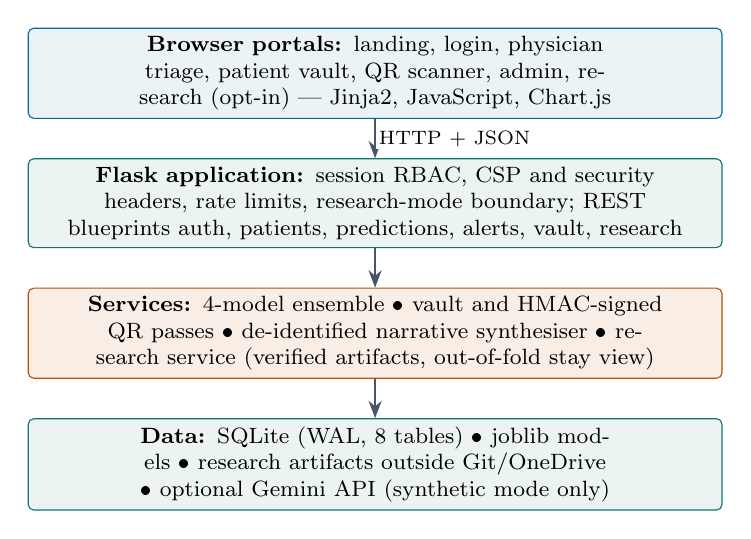
\begin{tikzpicture}[x=1mm, y=1mm, lay/.style={box, text width=86mm, font=\small, align=left, inner sep=4pt}]
\node[lay, blue box] (p) at (0,0) {\textbf{Browser portals:} landing, login, physician triage, patient vault,
QR scanner, admin, research (opt-in) \textemdash\ Jinja2, JavaScript, Chart.js};
\node[lay, teal box, below=5mm of p] (a) {\textbf{Flask application:} session RBAC, CSP and security headers,
rate limits, research-mode boundary; REST blueprints auth, patients, predictions, alerts, vault, research};
\node[lay, amber box, below=5mm of a] (s) {\textbf{Services:} 4-model ensemble \textbullet\ vault and
HMAC-signed QR passes \textbullet\ de-identified narrative synthesiser \textbullet\ research service
(verified artifacts, out-of-fold stay view)};
\node[lay, store, below=5mm of s] (d) {\textbf{Data:} SQLite (WAL, 8 tables) \textbullet\ joblib models
\textbullet\ research artifacts outside Git/OneDrive \textbullet\ optional Gemini API (synthetic mode only)};
\draw[flow] (p) -- node[lbl, right]{HTTP + JSON} (a);
\draw[flow] (a) -- (s);
\draw[flow] (s) -- (d);
\end{tikzpicture}
}
\end{pbox}
\begin{pbox}[Main Workflows]{mhblue}
\textbf{Triage:} roster $\rightarrow$ patient chart $\rightarrow$ consensus tier, each model's vote,
decision-tree rule path, similar cases, 72-h vitals.\\[1mm]
\textbf{Vault:} patient shares a pass (scope, lifetime $\le$ 30 days, uses) $\rightarrow$ clinician scans
$\rightarrow$ signature, expiry, revocation, \emph{atomic} use quota $\rightarrow$ only consented records,
access logged under the signed-in clinician.\\[1mm]
\textbf{Research (opt-in):} build dataset $\rightarrow$ grouped CV $\rightarrow$ hash-verified run
$\rightarrow$ analytics, what-if and stay-level triage with out-of-fold scores.
\end{pbox}
\begin{pbox}[Screens (synthetic data)]{mhteal}
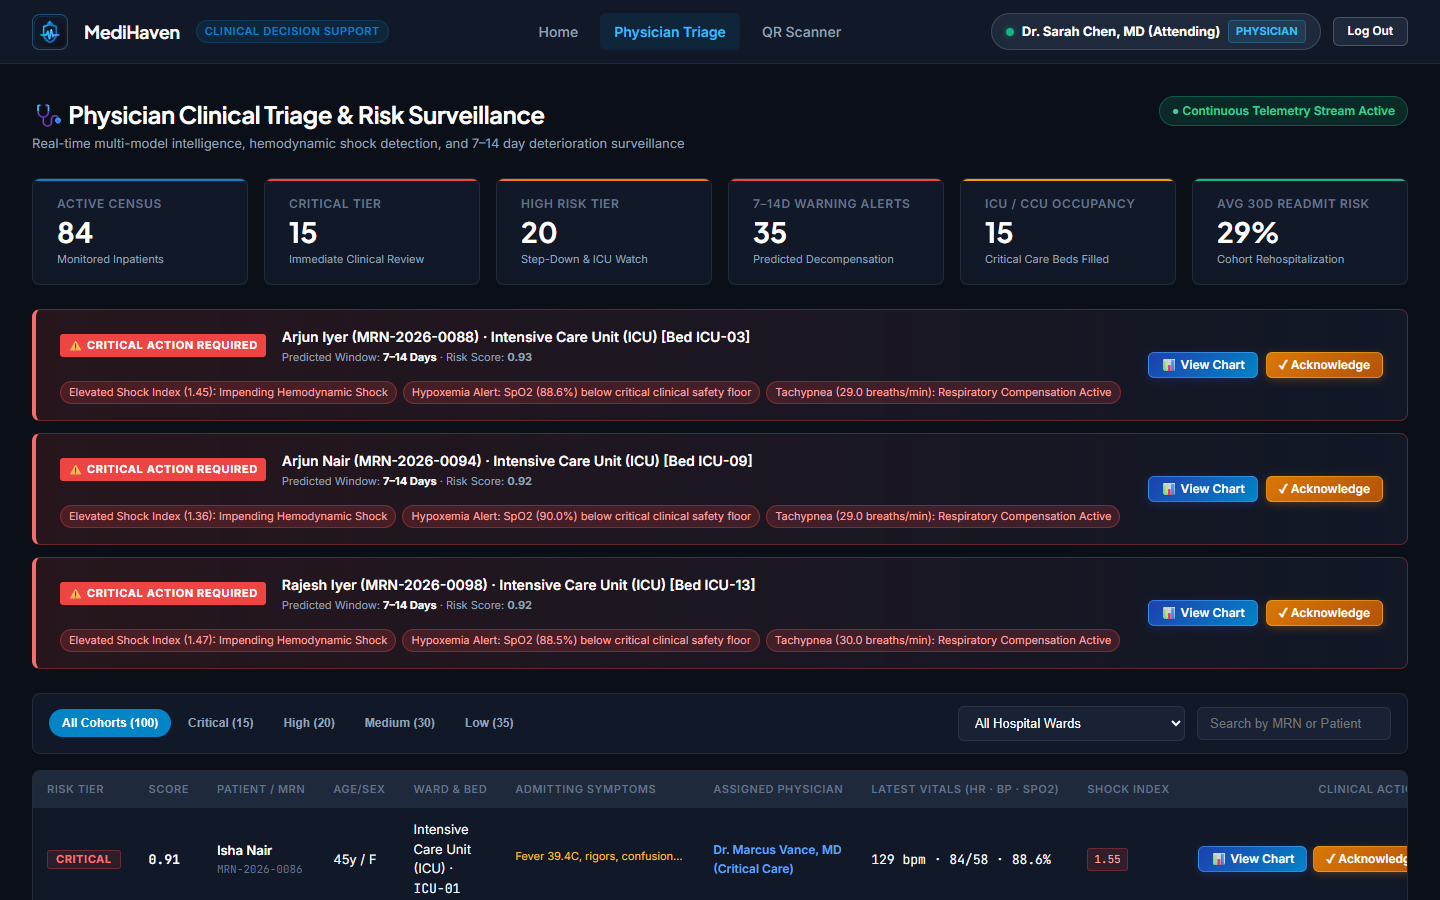
\includegraphics[width=0.49\linewidth]{../figures/screenshots/03_triage_dashboard.png}\hfill
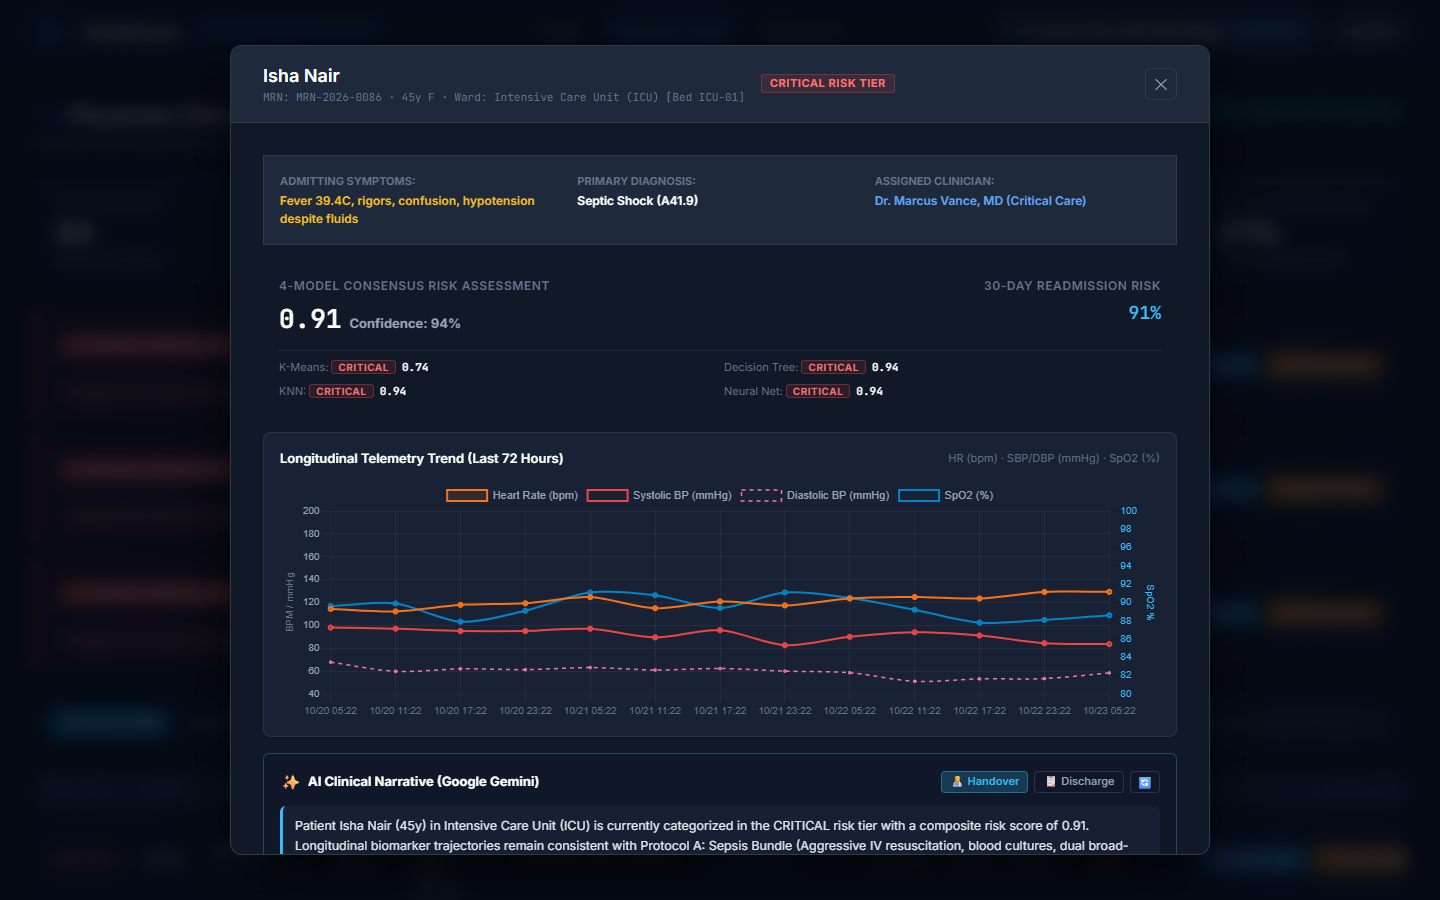
\includegraphics[width=0.49\linewidth]{../figures/screenshots/04_patient_chart_drawer.png}
\end{pbox}
\end{minipage}\hfill
\begin{minipage}[t]{0.245\linewidth}\vspace{0pt}
\begin{pbox}[Models]{mhamber}
\textbf{Synthetic ensemble} (4 tiers): weighted soft vote $0.30$ decision tree $+\,0.30$ MLP
$+\,0.25$ KNN $+\,0.15$ K-Means; tier $=\arg\max$, score $=\sum_t p_t s_t$.\\[1mm]
\textbf{Research baselines} (74 inputs from the first 24 ICU hours): prior-only reference, L2 logistic
regression, m-estimate-smoothed decision tree, random forest, small MLP; median imputation inside each fold.
\end{pbox}
\begin{pbox}[Research Results: 5-fold grouped CV, 95\% CI]{mhamber}
\centering
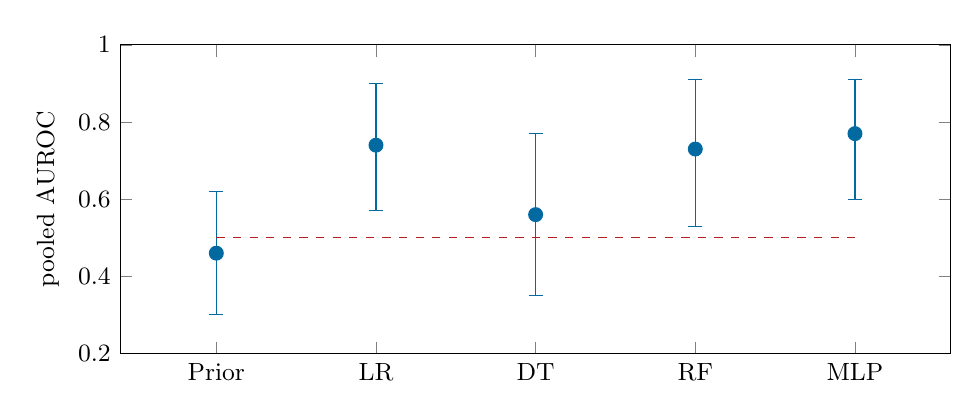
\begin{tikzpicture}
\begin{axis}[width=\linewidth, height=55mm, ylabel={pooled AUROC}, ymin=0.2, ymax=1.0,
  symbolic x coords={Prior,LR,DT,RF,MLP}, xtick=data, enlarge x limits=0.15,
  tick label style={font=\small}, label style={font=\small}]
\addplot[only marks, mark=*, mark size=2.5pt, mhblue, error bars/.cd, y dir=both, y explicit]
  coordinates {(Prior,0.46) += (0,0.16) -= (0,0.16) (LR,0.74) += (0,0.16) -= (0,0.17)
               (DT,0.56) += (0,0.21) -= (0,0.21) (RF,0.73) += (0,0.18) -= (0,0.20)
               (MLP,0.77) += (0,0.14) -= (0,0.17)};
\addplot[dashed, mhred] coordinates {(Prior,0.5) (MLP,0.5)};
\end{axis}
\end{tikzpicture}\\[1mm]
\raggedright
\small 107 stays, 11 deaths. Intervals overlap heavily; without the 4 anomalies (7 deaths, retrained)
LR and MLP fall to about 0.40. \textbf{Pipeline validation only, no clinical performance claim.}
Synthetic hold-out accuracy 1.00 reflects the data generator, not clinical skill.
\end{pbox}
\begin{pbox}[Research Mode Safeguards]{mhred}
Explicit opt-in (\texttt{DATA\_MODE=mimic}) \textbullet\ loopback only \textbullet\ strong secrets
enforced \textbullet\ SHA-256-verified artifacts \textbullet\ never calls Gemini \textbullet\ stays numbered,
no MIMIC identifiers or dates shown \textbullet\ research-only banners.
\end{pbox}
\end{minipage}\hfill
\begin{minipage}[t]{0.235\linewidth}\vspace{0pt}
\begin{pbox}[Testing]{mhteal}
\textbf{354 automated tests: 354 passed, 0 failed} (pytest, 26 Oct 2026): unit, API integration,
security, invalid-input, concurrency (4 simultaneous scans of a single-use pass $\rightarrow$ exactly 1
grant) and fail-closed research tests. Tests use temporary paths and never touch real data or secrets.
\end{pbox}
\begin{pbox}[Measured Performance (Waitress, 8 threads)]{mhteal}
\centering\small
\begin{tabular}{@{}lr@{}}
\toprule
Prediction latency, 1 client (p50) & 71.9 ms\\
Prediction throughput (saturated) & $\approx$15 req/s\\
Vitals reads, 16 clients & 268.8 req/s\\
Errors in 3{,}200 requests & 0\\
Server memory under load & $\le$ 206 MB\\
\bottomrule
\end{tabular}\\[1mm]
\raggedright Bottleneck: CPU-bound feature engineering + 4 models per prediction.
\end{pbox}
\begin{pbox}[Limitations and Intended Use]{mhred}
Synthetic data cannot show clinical validity; the real cohort is tiny and single-centre; calibration not
assessed; single-instance design; no browser end-to-end or penetration tests. For teaching and
demonstration only, never for diagnosis or treatment.
\end{pbox}
\begin{pbox}[Conclusion and Future Scope]{mhblue}
An integrated, tested and honest engineering prototype. \emph{Future work:} credentialed full MIMIC-IV
with external validation and calibration, feature caching and worker processes, shared state for scaling,
real document uploads, end-to-end and security testing.
\end{pbox}
\end{minipage}
\end{document}
